\section{\review{Resonances}}


%----------------------------------------
%             Tune Diagram
%----------------------------------------
\subsection{\review{Tune Diagram}}

The resonances discussed in this thesis are related to the optics of the accelerator.
Such resonances create unstable motion and can lead to loosing particles.
Those perturbations arise from particles oscillating at frequencies excited by certain multipoles.

\begin{figure}[!htb]
    \centering
    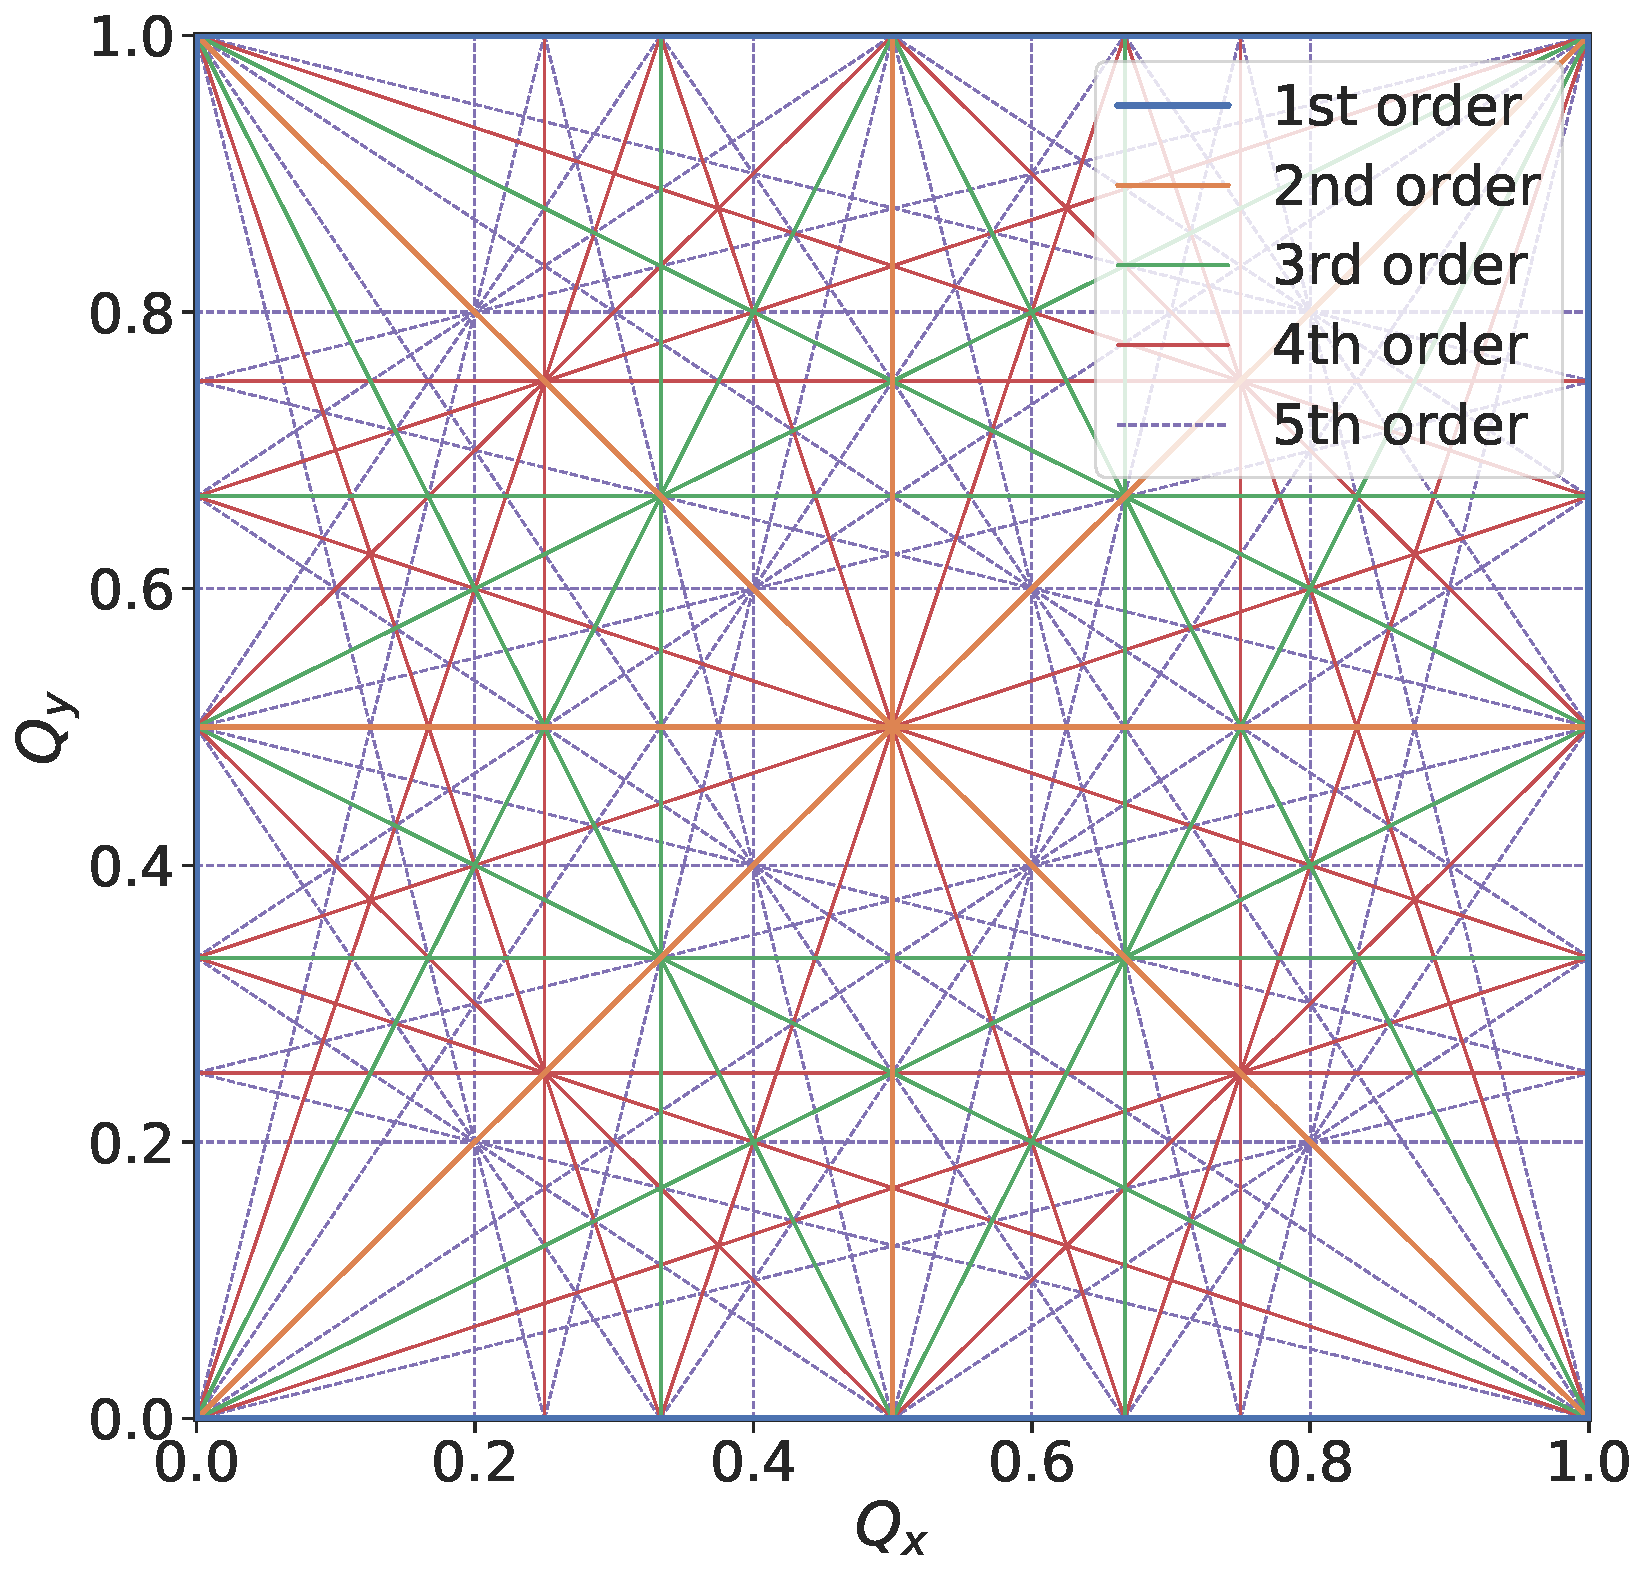
\includegraphics[width=0.82\textwidth]{images/resonance_diagram_n5.pdf}
    \caption{Tune diagram with resonances lines excited by multipoles up to decapole ($n \leq 5$).
             The working point of the machine is chosen in an area where few lines are present.}
    \label{fig:resonances:diagram_n5}
\end{figure}

\Cref{fig:resonances:diagram_n5} shows a tune diagram where the fractional part of tunes $Q_x$ and
$Q_y$ can be related to resonance lines excited by multipoles up to decapoles ($n=5$).
It becomes apparent that the diagram fills quickly when considering further orders.
%, as shows \cref{fig:resonances:diagram_n7}. 
Thankfully, the higher the multipole order, the weaker the resonances are. This makes choosing a
working point possible, even if some particles are hitting resonance lines.

%\begin{figure}[H]
%    \centering
%    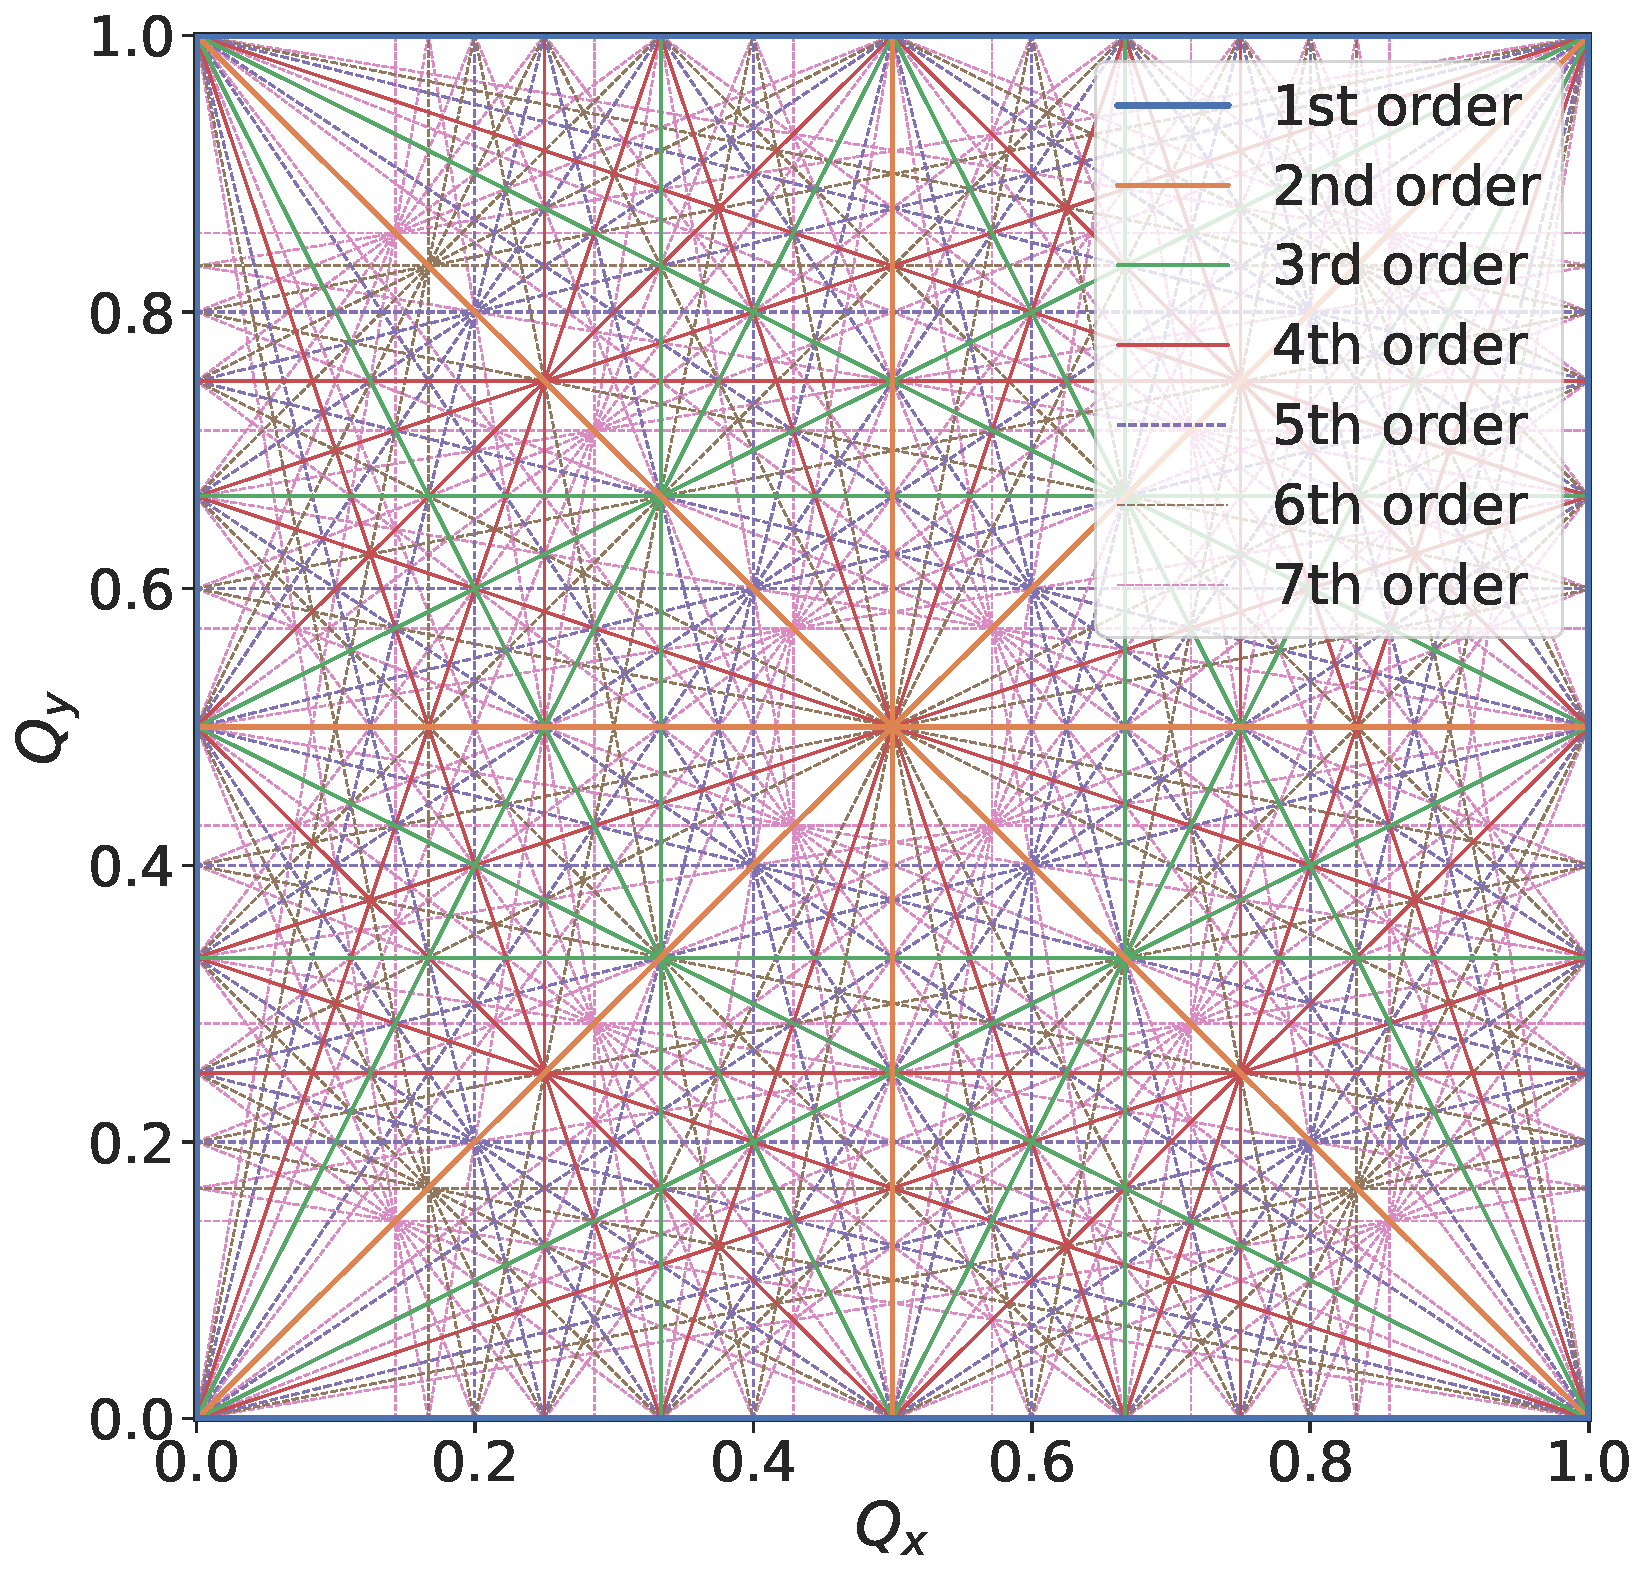
\includegraphics[width=0.82\textwidth]{images/resonance_diagram_n7.pdf}
%    \caption{Tune diagram with resonances lines excited by multipoles up to decatetrapole 
%             ($n \leq 7$). When considering higher orders, it becomes apparent that the beam will
%             inevitably hit several resonances.}
%    \label{fig:resonances:diagram_n7}
%\end{figure}


When considering the resonance driving terms $f_{jklm}$ from \cref{eq:coordinate_systems:fjklm}, it
can be noted that the term diverges for particular tune values. This leads to a disproportionate
increase in particles position in phase-space, eventually leading to loosing them.
Resonant conditions due to the tunes can thus be described by the following condition:

\begin{equation}
    (j-k)Q_x + (l-m)Q_y = p \quad,\quad j,k,l,m,p \in \mathcal{Z}.
\end{equation}
    


%----------------------------------------
%          Frequency Spectrum
%----------------------------------------
\subsection{\review{Frequency Spectrum}}

As seen in \cref{eq:coordinate_systems:linear_position_normal_form}, resonance driving terms have an
impact on the transverse position of a particle. This means that performing a FFT on such a signal
will reveal spectral lines in the frequency spectrum.
Each RDT $f_{jklm}$ can thus be observed in either one or both the frequency spectrums of the
horizontal and vertical planes, at multiples of $Q_x \pm Q_y$. \Cref{eq:resonances:rdt_spectrum}
shows where those lines would appear:

\begin{equation}
    \begin{aligned}
    & H_{jklm} \;&&\text{at}\; (1 - j + k)Q_x + (m - l)Q_y \quad&&; \quad j \ne 0 \\
    & V_{jklm}   &&\text{at}\; (k - j)Q_x + (1 - l + m)Q_y      &&; \quad l \ne 0.
    \end{aligned}
    \label{eq:resonances:rdt_spectrum}
\end{equation}

The RDT $f_{3000}$ coming from sextupoles can for example be seen in the horizontal spectrum at
$(1-3+0)Q_x + (0-0)Q_y = -2Q_x$. For a value $Q_x = 0.27$, the line is seen at $0.46$. in a spectrum
bound in $[0, 0.5]$. No line can be seen in the vertical spectrum due to $l = 0$.
Detailed tables of such lines for RDTs up to order 6 can be found in \cref{appendix:rdts}.

The amplitude of each line will depend on the action $I_z$ and the amplitude of the
RDT~\cite{bartolini_normal_1997}:

\begin{equation}
    \begin{aligned}
    |H_{f_{jklm}}| &= 2 j (2 I_x)^\frac{j+k-1}{2} (2 I_y)^\frac{l+m}{2} |f_{jklm}| \\
    |V_{f_{jklm}}| &= 2 l (2 I_x)^\frac{j+k}{2} (2 I_y)^\frac{l+m-1}{2} |f_{jklm}|.
    \end{aligned}
    \label{eq:resonances:amplitude_line}
\end{equation}


%----------------------------------------
%           RDT Calculation
%----------------------------------------
\subsection{\review{Resonance Driving Terms}}

By reworking the previous \cref{eq:resonances:amplitude_line}, it can be seen that RDTs are factors
of the line amplitude and the actions $I_x$ and $I_z$:

\begin{equation}
    \begin{aligned}
    |f_{jklm}| &= \frac{|H_{f_{jklm}}|}{2 j (2 I_x)^\frac{j+k-1}{2} (2 I_y)^\frac{l+m}{2}} \\
    |f_{jklm}| &= \frac{|V_{f_{jklm}}|}{2 l (2 I_x)^\frac{j+k}{2} (2 I_y)^\frac{l+m-1}{2}} .
    \label{eq:resonances:amplitude_rdt}
    \end{aligned}
\end{equation}

In practice, an approximation of $J = I$ is done. The RDT is then related to the fit of the line
amplitude versus the action.% as shown in \cref{fig:resonances:fit_rdt}.

%\begin{figure}[H]
%    \centering
%    \includegraphics[width=0.8\textwidth]{example-image-a}
%    \caption{.}
%    \label{fig:resonances:fit_rdt}
%\end{figure}